\chapter{Overview}

    There are diverse SDN controllers accessible. Some of them are open source ventures created and kept up by the network, while private associations build up a few. Notwithstanding open source or private, all controllers follow a similar rule of equipment autonomy and the partition and overcome approach. Similarly, as with any situation where there are numerous choices of a certain something, a decision is made in light of the fact that we can't send all the alternatives in a similar domain at the same time.
 
    To choose the best controller, first, there is a need to comprehend the idea of the best controller. What are the standards on which controllers should be judged or analysed? Is there even a potential best controller among them all. Like how we measure separation utilising a ruler, or time using a clock, we need a standard against which controllers can be thought about, and afterwards contrast the examinations and one another. This standard of measurements is urgent to choosing which controller would be perfect. There are a few papers which notice a couple of essential measurements, let us investigate.
    
   Controllers must be analyzed on a few models. Past papers talked about a wide assortment of properties of controllers going from physical execution to adaptation to internal failure. A portion of the measurements incorporate time for setting up the system, tearing down the system, preparing power Usage, potential to scale the system, CPU use, memory use, throughput, latency, ping delay, etc.
    
    These metrics give a fair idea of the performance of the controller on an industrial level. Nevertheless, all these criteria seem well researched and are continually evolving with upgraded hardware and new features in the software. Factors like system utilization also have to be evaluated to determine whether the controller uses the hardware constraints efficiently. It also gives a clear idea about the controller's nature while it is running and helps identify the system bottlenecks.
    
    A paper published in 2018 came up with methodologies for measuring the performance of all controller implementations and benchmarked the control- plane performance \cite{rfc8456}.
    
    Another paper, published in 2019, describes a repetitive series of tests using a network emulator and a benchmark tool that included the CPU utilization of various Controllers on a machine. It uses a benchmark tool which operates on a different system, that sends a considerable amount of random packets to the controller and then reads CPU utilization values. Fig. \ref{figzhu2019sdn} below depicts the average CPU utilization at a given time. The graph gets populated by data from the benchmark tool, which performs the test seamlessly. At the same time, the controller operating system runs on a virtual machine \cite{zhu2019sdn}. Currently, the benchmark OFNet used in that experiment is no longer available as the concerned owner has removed it.
    
    A paper, published in 2014, describes how OFCBench and OFCProbe can be used as CPU and RAM utilization monitor and find bottlenecks of the controller. The implementation of these monitors is by sending SMTP messages from client machines. However, it is worth noting that both these tools are limited to work with Floodlight, Ryu, and Nox Controllers. \cite{ofcprobe}
    
    One more paper, published in 2012, shows they used multiple instances of CBench to send packets and measure the CPU Utilization. They discovered an inherent performance bottleneck concerning CPU load in OpenFlow switch implementations of those days. \cite{flexible}
    
\begin{figure}[!hbt]
    \centering
        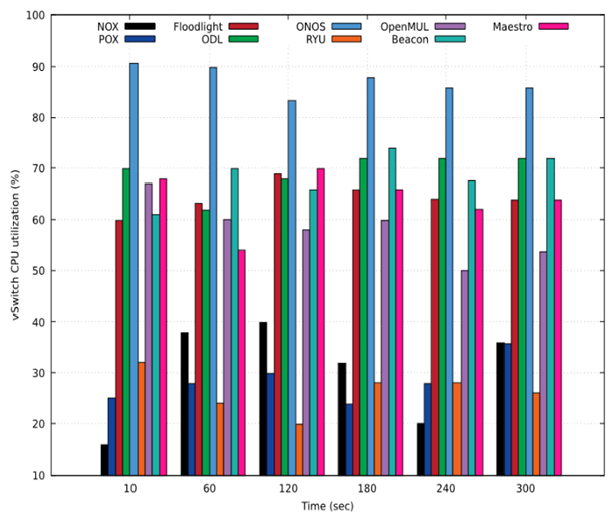
\includegraphics[width=\textwidth,keepaspectratio]{images/zhucpu.png}
       \caption{CPU Utilization Results Published \cite{zhu2019sdn}}
        \label{figzhu2019sdn}
\end{figure}

   The throughput method of CBench in which the switches are arranged to pause and heap up a lot of packets and send all the packets without a moment's delay to the controller. This powers the controller to dispense a huge portion of its resources to each or two switches in turn. This method gauges the pressure limit of the controller. The controller must have enough memory to store and procedure all the solicitations from a switch. It need not have the option to run such a large number of strings simultaneously.

        The tests acted in the paper \cite{dynamicrouting} think about numerous controllers, running in a system whose size increments. For this component, they expanded the number of hubs after each arrangement of tests and rehashed them while recording the outcomes. What appears to be neglected in this test is that the outcomes are legitimate, furnish us just with a fundamental thought of the controller's performance. The controller with the best development of the response rate in relation to organizing size was delegated the best controller.
        
    The controller provides more responses as the network size increase. It is because there is more packet in events from switches. As the network size increases, more routes need to be calculated and maintained. More switches need to be updated regularly. However, one factor is overlooked. The fact that more requests are generated is not necessarily because there are more switches; it is because there are more hosts overall connected to the network. The experiment performed as in paper \cite{routingtie2017} by increasing the number of switches while maintaining the number of hosts per switch. As the network grew, more hosts would want to communicate, thus leading to the rise in route requests or packet in events.
    
    \textit{Traffic Intensity} is a measure of how flooded a network is with traffic. As the network gets scaled up, the number of hosts increases, thus increasing traffic Intensity. This increase in traffic intensity forces the controller to increase its performance rates to cope with the network requirements. There is a need for a method to compare controller such that minimum external factors are influencing the controller's performance. Here, the traffic Intensity is kept quite high, changing the network topology to see how different controllers handle the scenario and how their performance is affected.

    For any test, the environment within which the subject to be tested must be isolated from external factors as much as possible. In the case of testing and performing a benchmark on SDN controllers, the cores of CPU where the controller runs, needs to be isolated using \textit{isolcpus} or similar tool.